\documentclass[10pt,a4paper]{article}
\usepackage[utf8]{inputenc}

\usepackage[english]{babel}

\usepackage{amsmath,amssymb}
\usepackage{amsthm,thmtools}
\numberwithin{equation}{section}
\declaretheorem[sibling=equation]{theorem}
\declaretheorem[sibling=equation]{proposition}
\declaretheorem[sibling=equation]{lemma}
\declaretheorem[sibling=equation]{definition}
\declaretheorem[sibling=equation,style=remark]{remark}
\declaretheorem[sibling=equation,style=remark]{idea}
\declaretheorem[sibling=equation]{conjecture}
\declaretheorem[sibling=equation]{notation}
\declaretheorem[sibling=equation]{example}
\declaretheorem[sibling=equation,style=remark]{exercise}
\newenvironment{solution}{}{}

\usepackage{enumitem}

\usepackage{tikz}
\usepackage{tikz-cd}

\newcommand{\ZZ}{\mathbb{Z}}
\newcommand{\QQ}{\mathbb{Q}}
\newcommand{\CC}{\mathbb{C}}
\newcommand{\FF}{\mathbb{F}}
\newcommand{\Aff}{\mathbb{A}}
\newcommand{\Spec}{\mathrm{Spec}}

\newcommand{\chr}{\mathrm{char}}

\newcommand{\nr}{\mathrm{nr}}

\usepackage[usenames,dvipsnames]{pstricks} 
\usepackage{epsfig}
\usepackage{graphicx,color}
\usepackage[all]{xy}
\xyoption{poly}
%\usepackage{calrsfs}
%\usepackage[T1]{fontenc}
%\usepackage{textcomp}

\title{Lecture notes on Berkovich skeleta}
\author{Johannes Nicaissen \and Sam Payne}

\begin{document}
\maketitle

\section{Lecture 1}

\subsection{Motivation}

To study the geometry of a complex variety $X/\CC$ it is often useful to put it
into a family and to study the other fibres
\[
	f \colon \mathfrak{X} \to \Aff^{1}_{\CC}
\]
such that $X \cong f^{-1}(a)$ for some $a$.

Typical situation: $X$ is smooth and proper over $\CC$. Then one might take
$\mathfrak{X}$ regular, $f$ proper and flat, and such that all singular fibres
of $f$ are strict normal crossings divisors.
(Strict normal crossings divisors means that locally they look like unions of
coordinate hyperplanes.)
\begin{center}
	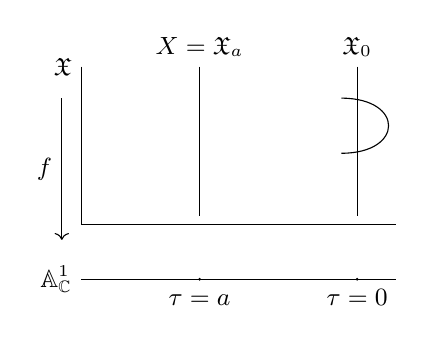
\begin{tikzpicture}[every node/.style={font=\small}]
		\draw (-2,2) node[left] {$\mathfrak{X}$} -- (-2,0) -- (2,0);
		\draw (-2,-.7) node[left] {$\Aff^{1}_{\CC}$} -- (2,-.7);
		\draw[->] (-2.25,1.6) -- node[left] {$f$} (-2.25,-.2);
		\draw (-.5,2) node[above] {$X = \mathfrak{X}_{a}$} -- (-.5,.1);
		\draw (1.5,2) node[above] {$\mathfrak{X}_{0}$} -- (1.5,.1);
		\draw (1.3,1.6) to [controls=+(0:.8) and +(0:.8)] (1.3,0.9);
		\draw[fill] (-.5,-.7) circle (.01) node[below] {$\tau = a\vphantom{0}$};
		\draw[fill] (1.5,-.7) circle (.01) node[below] {$\tau = 0$};
	\end{tikzpicture}
\end{center}
\begin{idea}
	The geometric complexity of $X$ is reflected in the geometric
	complexity of $\mathfrak{X}_{0}$.

	If we want to study the degeneration of the family at a particular
	fibre $\mathfrak{X}_{0}$, we can zoom in around $\mathfrak{X}_{0}$ by
	base changing to $\widehat{\mathcal{O}_{\Aff^{1}_{\CC,0}}} = \CC[[T]]$.

	So we want to study schemes over discrete valuation rings.
\end{idea}

\begin{notation}
	\begin{itemize}
		\item[$R$] discrete valuation ring
		\item[$t$] local uniformizer (i.e., generator of the maximal ideal)
		\item[$k$] residue field (we assume $k = \bar{k}$)
		\item[$K$] fraction field
	\end{itemize}
\end{notation}

\begin{example}
	There are two cases.
	\begin{itemize}
		\item The \emph{equal} characteristic case: $R = k[[t]]$, $K = k((t))$.
		\item The \emph{mixed} characteristic case: $R = \widehat{\ZZ_{p}^{\nr}} = W(\FF_{p})$, $K = \widehat{\QQ_{p}^{\nr}}$, $t = p$. (In general $R$ is a finite extension of $W(k)$.)
	\end{itemize}
\end{example}
The geometric picture corresponding to this is
\begin{itemize}
	\item[$\Spec(R)$] ``small disk around $0 \in \CC$''
	\item[$t$] ``coordinate on this disk''
	\item[$\Spec(K)$] ``small punctured disk around $0 \in \CC$''
\end{itemize}

Let $X$ be a smooth proper geometrically connected variety over $K$.
Geometrically we can think of a family of connected smooth proper varieties
over a punctured disk.
\begin{definition}
	A \emph{model for $X$ over $R$} is a proper and flat $R$-scheme $\mathfrak{X}$ together with an isomorphism $\mathfrak{X}_{K} \to X$.

	A morphism of models $\mathfrak{Y} \to \mathfrak{X}$ is an $R$-morphism such that
	\[
		\begin{tikzcd}[column sep=small]
			\mathfrak{Y}_{K} \ar{rr} \drar[near start,sloped]{\sim}
			&& \mathfrak{X}_{K} \dlar[near start,swap,sloped]{\sim} \\
			& X
		\end{tikzcd}
	\]
	commutes.
\end{definition}
Note: There exists at most one morphism from $\mathfrak{Y}$ to $\mathfrak{X}$.
If such a morphism exists, we say that $\mathfrak{Y}$ dominates $\mathfrak{X}$.
We say that $\mathfrak{X}$ is an \emph{snc-model} if $\mathfrak{X}$ is regular
and $\mathfrak{X}_{k}$ is a strict normal crossings divisor, i.e., for every $x
\in \mathfrak{X}$, there exists a regular system of local parameters
\emph{(i.e., a basis of the Zariski tangent space)} $(Z_{1}, \ldots Z_{d})$ and
a unit $u$ in $\mathcal{\mathfrak{X},x}$ such that $t = uZ_{1}^{N_{1}} \cdots
Z_{d}^{N_{d}}$ for some $N_{i} \ge 0$. We say that $\mathfrak{X}$ is an
\emph{nc-model} if $\mathfrak{X}$ is regular and $\mathfrak{X}_{k}$ is a normal
crossings divisor, i.e., an snc-divisor for the étale topology. This ``allows
for self-intersections''.
\begin{center}
	\begin{tikzpicture}[every node/.style={font=\small}]
		\draw (0,0) to [controls=+(110:3) and +(250:3)] (0,1);
		\path (0,.5) node[right] {nc, but not snc};

		\draw[->] (-.5,-1.2) -- node[right] {étale} (-.5,-.4);

		\begin{scope}[yshift=-2.5cm]
			\draw (0,0) to [controls=+(180:1) and +(180:1)] (0,1);
			\draw (0,.1) to [controls=+(200:2) and +(160:2)] (0,.9);
		\end{scope}
	\end{tikzpicture}
\end{center}

The variety $X$ always has an $R$-model, by Nagata's embedding theorem.
\[
	\begin{tikzcd}
		X \dar{\text{proper}} \rar[hook]{\exists} & \mathfrak{X} \dar \\
		\Spec(K) \rar[hook] & \Spec(R)
	\end{tikzcd}
\]
The existence of nc-/snc-models is much more subtle and relies on
\emph{resolution of singularities}. This is expected to be true in general by
most experts; but currently we know:
\begin{itemize}
	\item $\chr(k) = 0$: holds for all $X$ (Hironaka, 1964)
	\item $\chr(k) > 0$: holds if $\dim(X) = 1$ (Lipman, 1978)
	\item $\chr(k) > 0$: holds if $\dim(X) = 2$ (Cossart--Pikant, last week?)
\end{itemize}
Until further notice, we will assume $\dim(X) = 1$.

\subsection{Intersection theory}

Intersection theory over discrete valuation rings (Lichtenbaum).

Let $X$ be a curve, $\mathfrak{X}$ a regular model of $X$. A divisor $E =
\sum_{i=1}^{n} a_{i}E_{i}$ is \emph{vertical} if it is supported on
$\mathfrak{X}_{k}$. (In particular, then $E$ is proper over $k$.)

\begin{figure}
	\caption{The distinction between horizontal and vertical divisors}
	\label{horvertdivs}
	\begin{center}
		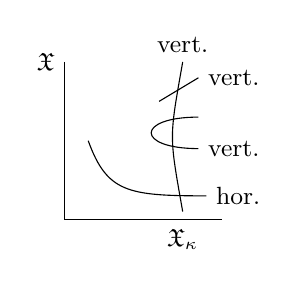
\begin{tikzpicture}[every node/.style={font=\small}]
			\draw (0,2) node[left] {$\mathfrak{X}$} -- (0,0) -- (2,0);
			\draw (1.5,2) node[above] {vert.} to[controls=+(260:1) and +(100:1)] (1.5,.1);
			\draw (1.2,1.5) -- (1.7,1.8) node[right] {vert.};
			\draw (1.7,1.3) to [controls=+(180:.8) and +(180:.8)] (1.7,0.9) node[right] {vert.};
			\draw (.3,1) to[controls=+(290:.7) and +(180:1)] (1.8,.3) node[right] {hor.};
			\path (1.5,0) node[below] {$\mathfrak{X}_{\kappa}$};
		\end{tikzpicture}
	\end{center}
\end{figure}

Let $E = \sum_{i=1}^{n} a_{i}E_{i}$ be a vertical divisor, and $D$ any divisor.
The intersection product is defined as:
\[
	(D \cdot E) = \sum_{i=1}^{n} a_{i} \deg \mathcal{O}(D)|_{\tilde{E_{i}}},
\]
where $\tilde{E_{i}} \to E_{i}$ is the normalisation.

The intersection product has the following properties:
\begin{itemize}
	\item It coincides with the geometric intuition if $D$ and $E$ have no common components.
	\item It is bilinear.
	\item It is symmetric if $D$ is vertical.
	\item It is invariant under linear equivalence on $D$.
	\item It is \emph{not(!)} invariant under linear equivalence on $E$.
		For example $\mathfrak{X}_{k} \sim 0$, but $(D \cdot
		\mathfrak{X}_{k}) \ne 0$ if $D$ consists of one horizontal
		component. See for example \cref{horvertdivs}.
	\item Behaviour under morphisms: If $h \colon \mathfrak{Y} \to
		\mathfrak{X}$ is a morphism of models, then
		\begin{center}
			\begin{tabular}{ll}
				$(D \cdot h^{*}E) = (h_{*}D \cdot E)$ &
				$(h^{*}D \cdot E) = (D \cdot h_{*}E)$ \\
				$D$ on $\mathfrak{Y}$ & $D$ on $\mathfrak{X}$ \\
				$E$ vertical on $\mathfrak{X}$ & $E$ vertical on $\mathfrak{Y}$
			\end{tabular}
		\end{center}
		which also imply $(h^{*}D \cdot h^{*}E) = (D \cdot E)$, when
		$D$ is a divisor on $\mathfrak{X}$, and $E$ a vertical divisor
		on $\mathfrak{X}$.
\end{itemize}

If $D$ is a divisor on a regular model $\mathcal{X}$ of $X$, then 
\[
(D \cdot \mathcal{X}_{k}) = \mathrm{deg}(D|_{X}).
\]
\begin{exercise}
	Prove this.
\end{exercise}

\section{Lecture 2}

\subsection{Minimal models}

A regular model


\section{Lecture 3}

\section{The semistable reduction theorem (Lecture 4)}

\noindent {\bfseries Recall} An nc-model for $X$ is called semistable if the special fibre is reduced.

\begin{definition} We say that $X$ has semistable reduction if it has a semistable nc-model. In that case, every relatively minimal nc-model will be semi-stable. \end{definition}
\begin{exercise} Prove the last statement. \end{exercise}

\noindent These models play an important role in the study of moduli spaces of curves (cf. Deligne--Mumford).

\begin{remark} An important feature is that it is easy to understand the behaviour of semistable nc-models under base change:

Let $\mathcal{X}$ be a semistable nc-model of $X$. Consider singular points of $\mathcal{X}_k$. I.e., let components $E_1$ and $E_2$ meet in a node, parametrised by the equation $xy=t$, for $t$ a uniformiser in $R$. Let $K'/K$ be a finite field extension of degree $d$ and let $R'$ be an integral closure of $F$ in $K'$; then $R'$ is again a complete discrete valuation ring. Now consider
\[
\mathcal{X}' = \mathcal{X} \times_R R'.
\]
This $\mathcal{X}'$ is no longer semistable: so-called $A_d$-{\emph singularities} appear. These are points where components $E_1$ and $E_2$ meet in a singular point parametrised by $x'y' = (t')^d$, where $t'$ is a uniformiser in $R'$.

%TO DO: Include pictures of the nodes in $\mathcal{X}_{k}$ and $\mathcal{X}'_k$ respectively.
{\bfseries N.B.} The extension $K'/K$ is totally ramified since we have assumed that $k$ is algebraically closed.

There is a minimal resolution of the $A_d$-singularieties, which will yield a new nc-model: Between $E_1$ and $E_2$ we introduce a chain of $d$ rational curves. On the level of dual graphs, this means that the edge between $v_1$ and $v_2$ (corresponding to $E_1$ and $E_2$ respectively) is subdivided into $d$ edges.
%TO DO: Include picture of a chain of d rational curves between components E_1 and E_2, and a dual picture of the graph with subdivided egde.
\end{remark}

\begin{theorem}[Semistable Reduction Theorem, Deligne--Mumford/Artin--Winters/Saito]
There exists a finite separable extension $K'/K$ such that $X \times_K K'$ has semistable reduction. More precisely, if $g(X) \neq 1$ or $X$ is an elliptic curve, then $X$ has semistable reduction if and onlly if the action of $\mathrm{Gal}(K^{\mathrm{sep}}/K)$ on $H^1(X\times_K K^{\mathrm{sep}},\mathbb{Q}_{\ell})$ is unipotent, i.e., has all eigenvalues equal to $1$.\end{theorem}

\begin{proof} The proof is elementary if $X$ has an nc-model $\mathcal{X}$ such that $\chr(k)$ does not divide the multiplicity of any component in $\mathcal{X}_k$.

A component $E$ of $\mathcal{X}_k$ is called \emph{principal} if $g(E) \geq 1$, or $E$ intersects the other components in at least $3$ points. (I.e., the components which are not principal are $\mathbb{P}^1$'s meeting in at least $3$ points.)

Let $$e = \mathrm{lcm}\{N_i \colon i \in I, E_i \textrm{  principal}\}$$ and write $$\mathcal{X}_k = \sum_{i \in I}N_iE_i.$$ Let $K'$ be the unique degree $e$ extension of $k$ in $K^{\mathrm{sep}}$, i.e., $K' = K(\sqrt[e]{t})$ where $t$ is a uniformiser in $R$. Let $R'$ again denote the integral closure of $R$ in $K'$.

For the normalisation $\widetilde{\mathcal{X} \times_R R'}$, which has only $\ZZ/e\ZZ$-quotient singularities by assumption. Its minimal resolution $\mathcal{Y}$ is an snc-model of $X \times_K K'$ but need not be semistable. When we contract its exceptional curves, we \emph{do} obtain a relatively minimal snc-model, $\mathcal{Y}'$ say, which is semistable.
\[
\xymatrix{
\widetilde{\mathcal{X}\times_R R'} \ar[d]_{\mathrm{normalisation}} & \ar[l]^{\mathrm{min. res.}} \mathcal{Y} \ar[d]^{\textrm{contract exceptional curves}} \\
\mathcal{X} & \mathcal{Y}' 
}
\]
If $\mathcal{X}$ is minimal, then $e$ is the degree of the smallest extension $K'$ such that $X \times_K K'$ has semistable reduction.

This strategy fails in general! Wild quotient singularities may appear on $\widetilde{\mathcal{X} \times_R R'}$. There is no general formula to compare the degree of the minimal extension giving a semi-stable reduction.

Note also that this theorem and its proof make heavy use of the fact that we are dealing with curves.
\end{proof}

\section*{Canonical divisor and adjunction formula}
Let $\mathcal{X}$ be a regular model of $X$. Write $\omega_{X/K} = \Omega^1_{X/K}$ for the canonical line bundle. This line bundle has a canonical extension to a line bundle on $\mathcal{X}$, called the \emph{relative canonical line bundle} $\omega_{\mathcal{X}/R}$. It is constructed (cf. Liu, "Algebraic Geometry and Arithmetic Curves") as $$\omega_{\mathcal{X}/R} = \mathrm{det}\Omega^1_{\mathcal{X}/R},$$ where $\mathrm{det}$ is the maximal exterior power of any locally free sheaf.

\noindent {\bfseries Why is the relative canonical line bundle important?}
\begin{enumerate}
\item $\omega_{\mathcal{X}/R}$ is a dualising sheaf, used in Grothendieck-Serre duality.
\item We have the {\bfseries Adjunction Formula}: $$\omega_{\mathcal{X}/R}|_X \cong \omega_{X/K}.$$ If $E$ is a prime component in $\mathcal{X}_k$ (i.e. one of the $E_i$ in $\mathcal{X}_k = \sum_{i} N_iE_i$), then $$\omega_{\mathcal{X}/R}(E)|_E \cong \omega_{E/k}.$$ Since $\omega_{E/k}$ has degree $2p_a(E) -2$, taking degrees on both sides yields $$p_a(E) = 1 + \frac{1}{2}((K_{\mathcal{X}/R} + E)\cdot E),$$ where $K_{\mathcal{X}/R}$ is any divisor associated with $\omega_{\mathcal{X}/R}$.
\end{enumerate}

\section*{A combinatorial toolbox}
Let $\mathcal{X}$ be an snc-model of $X$ and write $\mathcal{X}_k = \sum_{i \in I} N_i E_i$. We have the invariants $$\kappa_i = -(E_i \cdot E_i)$$ and $$\nu_i = (K_{\mathcal{X}/k}\cdot E_i).$$ %Should the k be an R??
These satisfy three fundamental relations:
\begin{enumerate}
\item $$\sum_{i \in I} N_i (E_i \cdot E_j) = 0$$ for all $j \in I$. This allows us to compute the $K_j$ on $\Gamma(\mathcal{X}_k)$.
\item (Adjunction Formula) $$2g(E_i)-2 = \nu_i - \kappa_i$$ for all $i \in I$. Note that here $g = p_a$, since all components are regular. This relations allows us to compute the $\nu_i$ on $\Gamma(\mathcal{X}_k)$.
\item $$2g(X)-2 = \mathrm{deg}\omega_{X/K} = (\omega_{\mathcal{X}/R} \cdot \mathcal{X}_k) = \sum_{i \in I} N_i \nu_i.$$ This allows us to compute the genus $g(X)$ on $\Gamma(\mathcal{X}_k)$. Note that only the horizontal part of $\omega_{\mathcal{X}/R}$ contributes.
\end{enumerate}

\begin{exercise} Write the adjunction formula in terms of $\Gamma(\mathcal{X}_k)$ if $\mathcal{X}$ is semistable. \end{exercise}


\section{Jacobians of graphs I (Lecture 5)}
Let $X$ be a smooth projective curve over $\mathbb{C}((t))$. Let $\mathcal{X}$ be a regular semistable snc-model and $G$ the dual graph of $\overline{\mathcal{X}} = \mathcal{X}_{\mathbb{C}}$.

The restriction map $\mathrm{Pic}(\mathcal{X}) \to \mathrm{Pic}(X)$ has a kernel generated by $\mathcal{O}(\overline{\mathcal{X}}_i)$, where $\overline{\mathcal{X}} = \overline{\mathcal{X}}_0 \cup \ldots \cup \overline{\mathcal{X}}_n$ with all $\overline{\mathcal{X}}_i$ irreducible.

Let $L$ be a line bundle on $X$. Let $\mathcal{L}$ be a model of $L$; then $\mathcal{L}$ is a line bundle on $\mathcal{X}$ and $\mathcal{L}|_X \cong L$.

Consider the matrix $\Delta$ such that $\Delta_{ij} = \mathrm{deg}(\mathcal{O}(\overline{\mathcal{X}}_i)|_{\overline{\mathcal{X}}_j})$. Note: if $i \neq j$ then $$\Delta_{ij} = \#(\overline{\mathcal{X}}_i \cap \overline{\mathcal{X}}_j) = \#(\textrm{edges from } v_i \textrm{ to } v_j \textrm{ in } G).$$
Alsno note that $\Delta_{ii} = -\mathrm{deg}(v_i) = \#(\textrm{outgoing edges})$. Hence, $$\Delta = -\mathrm{Deg} + \mathrm{Adj},$$ the so-called \emph{combinatorial Laplacian} of $G$.

The degree map is defined by $$\mathrm{deg} \colon \mathrm{Pic}(\mathcal{X}) \to \mathbb{Z}^{n+1} \colon \mathcal{L} \mapsto (\mathrm{deg}(\mathcal{L}|_{\overline{\mathcal{X}}_0}),\ldots, \mathrm{deg}(\mathcal{L}|_{\overline{\mathcal{X}}_n})).$$
Two different models of $L$, say $\mathcal{L}$ and $\mathcal{L}'$, satisfy $\mathrm{deg}(\mathcal{L}) - \mathrm{deg}(\mathcal{L}) \in \mathrm{Im}(\Delta)$, when we view $\Delta$ as a map $\Delta \colon \mathbb{Z}^{n+1} \to \mathbb{Z}^{n+1}$.

This yields a well-defined map $\tau_{*}$, fitting into a commutative diagram
\[
\xymatrix{
\mathrm{Pic}(X) \ar[r]^{\tau_{*}} \ar[dr]^{\mathrm{deg}} & \mathbb{Z}^{n+1}/\mathrm{Im}(\Delta) \ar[d]^{[(a_0,\ldots,a_n)] \mapsto a_0 + \ldots + a_n} \\
 & \mathbb{Z} 
}
\]
We have $\mathrm{ker}(\mathrm{deg}) = (\mathbb{Z}^{n+1}/\mathrm{Im}(\Delta))_{\mathrm{tors}} =\colon \mathrm{Jac}(G)$ and we know that $\Delta$ has rank $n$.

\begin{exercise}[The Matrix Tree Theorem]
	Show that
	\[
		\#\mathrm{Jac}(G) = \#\{\text{spanning trees of } G\}.
	\]
\end{exercise}

\begin{definition} For the semigroup $\mathrm{Eff}(X) \subseteq \mathrm{Pic}(X)$ generated by $\mathcal{O}(x)$ for $x \in X$, we have $\tau_{*}\mathrm{Eff}(X) \subseteq \mathbb{Z}^{n+1}_{\geq 0} = \colon \mathrm{Eff}(G)$. Then we define $\mathrm{Pic}(G) \colon = (\mathbb{Z}^{n+1}/\mathrm{Im}(\Delta))$.

So $\mathrm{Eff}_1(G) = [v_i],\ldots$, $\mathrm{Eff}_2(G) = [v_i + v_j], \ldots$ and in general, $\mathrm{Eff}_d(G) = \{ [a_0 v_0 + \ldots + a_nv_n] \colon a_i\geq 0, a_0 + \ldots + a_n = d \}$. \end{definition}

\begin{remark} Recall: for $D$ a divisor on $X$, its rank satisfies $r(D) = h^0(\mathcal{O}(D)) - 1 = \mathrm{dim}|D|$. Thus, $r(D)$ is the largest integer $r$ such that for every $E \in \mathrm{Eff}_r(X)_{\overline{\mathbb{C}((t))}}$ we have $[D-E] \in \mathrm{Eff}(X)$. N.B.: For this to hold, we need the ground field to be algebraically closed.\end{remark}

\begin{definition}[Baker-Norine, 2007] For $D = a_0v_0 + \ldots a_n v_n$ a divisor on $G$, $r([D])$ is the largest integer $r$ such that for all $E \in \mathrm{Eff}_r(G)$, $[D-E]$ is contained in $\mathrm{Eff}(G)$. \end{definition}

\begin{remark} If $D$ is not effective, then $r(D) = -1$, and conversely. \end{remark}

\begin{lemma}[Specialisation Lemma, Baker 2008] The rank satisfies $$r(\tau_{*}([D])) \geq r([D])$$ for $D \in \mathrm{Div}(X)$.\end{lemma}
This lemma allows us to "prove theorems on curves by looking at the graphs".

\begin{definition}[S.W. Zhang, 1990] The \emph{canonical divisor on a graph} is given by $$K_G = \sum_v (\mathrm{deg}(v)-2)\cdot v.$$ \end{definition}

\begin{remark} If every component of $\mathcal{X}$ is a $\mathbb{P}^1$, then $K_G = \sum_i \mathrm{deg}(K_{\mathcal{X}}|_{\overline{\mathcal{X}}_i})\cdot \nu_i$. \end{remark}

\begin{theorem}[Tropical Riemann-Roch, Baker-Norine] If $D = a_0 v_0 + \ldots + a_n v_n$ then $$ r([D]) - r([K_G-D]) = \mathrm{deg}(D) + 1 -g,$$ where $g = h^1(G) = e-v+1$ is the first Betti number of the graph, which equals $g(X)$ if $\overline{\mathcal{X}}_1 \cong \mathbb{P}^1$.\end{theorem}

\subsection{Open problems}
\begin{enumerate}
\item Does the Riemann-Roch theorem for curves imply the tropical Riemann-Roch theorem, or conversely?
\item Is there a unified proof of the Riemann-Roch for curves and the tropical Riemann-Roch? Would this be easier?
\end{enumerate}

\subsection{Some remarks}
\begin{enumerate}
\item There are analogues of rank, tropical Riemann-Roch and the specialisation lemma for $g(\mathcal{X}_i) > 0$, by work of Amini and Caporaso (Advances, 2013 or 2014).
\item We could also use metrised complexes (i.e. a simplicial realisation of the special fibre with a metric on the edges), by work of Amini and Baker (to appear in Math. Annalen).
\end{enumerate}

\subsection{Some more exercises}
\begin{exercise} Compute $\mathrm{Jac}(G)$ for $G = \ldots$ 
%TO DO: Include pictures of a triangular graph, a square, and a triangle attached to a square
\end{exercise}
%\begin{solution} $\ZZ/3\ZZ$, $\ZZ/4\ZZ$, $\ZZ/11\ZZ$.
%\end{solution}
\begin{exercise} Show that the map $\mathbb{Z}^{\mathrm{vert}(G)} \to \mathrm{Jac}_{\mathbb{R}}(G)$ vanishes on $\mathrm{Im}(\Delta)$. \end{exercise}
%\begin{solution}
%\end{solution}


\section{Lecture 6}
\section{Lecture 7}
\section{Lecture 8}
\section{Lecture 9}
\section{Lecture 10}
\section{Lecture 11}
\section{Lecture 12}
\section{Lecture 13}
\section{Lecture 14}
\section{Lecture 15}

\end{document}
